%-----------------------------------------------------------------------------%
\chapter{\babDua}
\label{cha:Tinjauan Pustaka}
%-----------------------------------------------------------------------------%
Bab ini menjelaskan konteks dan landasan teoretis yang mendasari penelitian mengenai analisis sinyal EEG untuk klasifikasi \textit{Autism Spectrum Disorder} (ASD) menggunakan metode \textit{machine learning}. Penjelasan diawali dengan pemaparan landasan teori, dilanjutkan dengan pembahasan penelitian terdahulu yang relevan, dan diakhiri dengan pembahasan mengenai celah penelitian yang menjadi dasar penelitian ini.
\section{Landasan Teori}
\label{sec:landasan_teori}
Bagian ini menguraikan konsep-konsep teoretis yang menjadi dasar dalam penelitian analisis sinyal EEG untuk klasifikasi Autism Spectrum Disorder (ASD). Landasan teori ini mencakup konsep dasar EEG, tahapan pemrosesan sinyal EEG, teknik seleksi fitur dalam pemrosesan, metode \textit{machine learning} untuk klasifikasi, serta metode \textit{data augmentation} yang digunakan dalam penelitian ini.

\subsection{Sinyal EEG}
\label{Konsep Dasar Sinyal EEG}

Sinyal \textit{electroencephalogram} (EEG) dihasilkan oleh aktivitas listrik neuron di otak yang muncul akibat aktivitas sinaptik antar neuron, sehingga potensial listrik yang dihasilkan dapat dideteksi pada permukaan kepala menggunakan elektroda. Sinyal EEG direkam sebagai perubahan tegangan terhadap waktu dengan rentang frekuensi sekitar 0,5 hingga 100 Hz dan amplitudo yang relatif rendah, umumnya berada pada kisaran 10 hingga 100 mikrovolt. Selain memiliki resolusi temporal yang tinggi, sinyal EEG juga bersifat \textit{non-stationary}, sehingga karakteristik amplitudo dan distribusi frekuensinya dapat berubah secara dinamis seiring waktu akibat pengaruh kondisi fisiologis, tingkat kesadaran, maupun aktivitas kognitif. Aktivitas yang terekam mencerminkan berbagai proses otak, seperti fungsi kognitif, motorik, dan emosional, sehingga EEG banyak digunakan untuk mempelajari fungsi otak dan gangguan neurologis \cite{eeg_basics}.

EEG biasanya direkam dalam bentuk sinyal multikanal yang diperoleh dari sejumlah elektroda yang ditempatkan pada berbagai lokasi di permukaan kulit kepala. Setiap kanal merepresentasikan satu jalur perekaman sinyal yang berasal dari pasangan elektroda atau dari elektroda terhadap referensi tertentu. Setiap elektroda menangkap aktivitas listrik dari wilayah otak yang berbeda, sehingga setiap kanal mengandung informasi yang merepresentasikan aktivitas saraf pada lokasi tertentu.\cite{eeg_feature_review}.


Penempatan elektroda EEG umumnya mengikuti standar International \textit{10–20 System}, yaitu protokol yang distandarisasi oleh \textit{International Federation of Clinical Neurophysiology} (IFCN) untuk menentukan posisi elektroda pada permukaan kepala berdasarkan titik anatomi seperti nasion, inion, dan titik preauricular. Dalam sistem ini, setiap elektroda diberi kode huruf dan angka yang menunjukkan wilayah otak dan hemisfer terkait, seperti frontal (F), central (C), temporal (T), parietal (P), dan occipital (O), dengan angka ganjil untuk hemisfer kiri, angka genap untuk hemisfer kanan, serta ``z'' untuk posisi garis tengah kepala. Tata letak elektroda pada sistem ini ditunjukkan pada Gambar \ref{fig:2.1}. Standarisasi ini memungkinkan perekaman EEG dilakukan secara konsisten dan dapat dibandingkan antar subjek maupun antar penelitian\cite{eeg_biophysics}.

\begin{figure}[H]
    \centering
    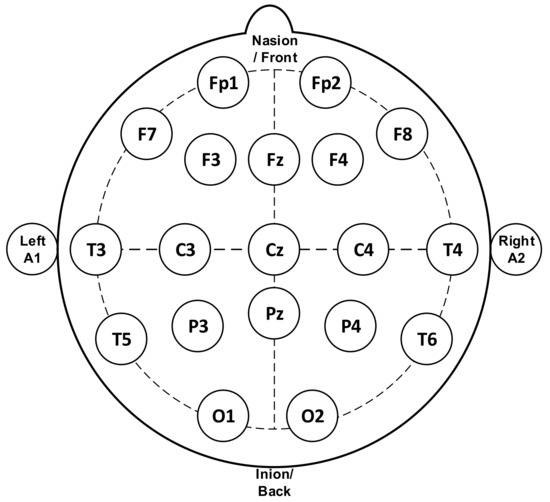
\includegraphics[width=0.6\textwidth]{assets/pics/10_20_system.jpg}
    \caption{Sistem Internasional 10--20 untuk penempatan elektroda EEG}
    \label{fig:2.1}
\end{figure}

Dalam analisis sinyal EEG, aktivitas listrik otak yang terekam dapat dianalisis melalui dua domain utama, yaitu domain waktu dan domain frekuensi. Analisis dalam domain waktu dilakukan dengan mengamati karakteristik sinyal terhadap waktu, seperti amplitudo puncak, dan latensi. Sedangkan analisis dalam domain frekuensi bertujuan untuk mengidentifikasi kandungan spektral sinyal dengan memeriksa distribusi energi atau daya pada berbagai rentang frekuensi menggunakan metode transformasi spektral, seperti \textit{Fast Fourier Transform} (FFT) maupun teknik estimasi \textit{Power Spectral Density} (PSD) untuk mengidentifikasi aktivitas otak pada rentang frekuensi tertentu \cite{auditory_eeg}.

Dalam analisis spektral EEG, sinyal umumnya dibagi ke dalam beberapa segmen waktu (\textit{epoch}) sebelum dihitung nilai \textit{Power Spectral Density} (PSD) untuk menggambarkan distribusi daya pada setiap frekuensi. Berdasarkan karakteristik fisiologis dan kognitifnya, sinyal EEG kemudian diklasifikasikan ke dalam beberapa pita frekuensi utama seperti pada tabel \ref{tab:eeg_bands}.

\begin{table}[H]
\centering
\footnotesize
\caption{Pita frekuensi EEG dan karakteristiknya}
\label{tab:eeg_bands}
\begin{tabular}{|c|c|p{8cm}|}
\hline
\textbf{Pita} & \textbf{Frekuensi (Hz)} & \textbf{Karakteristik} \\ \hline
Delta & 0,5--4 & Dominan pada kondisi \textit{deep sleep} dan berperan dalam proses pemulihan fisiologis serta regulasi fungsi tubuh selama tidur. \\ \hline
Theta & 4--8 & Berkaitan dengan proses pembentukan memori dan aktivitas pada sistem limbik serta hipokampus, serta muncul pada kondisi mengantuk atau relaksasi mendalam. \\ \hline
Alpha & 8--13 & Muncul pada kondisi rileks saat mata tertutup, dengan dominasi pada wilayah oksipital dan berhubungan dengan penurunan aktivitas pemrosesan sensorik. \\ \hline
Beta & 13--30 & Berkaitan dengan aktivitas kognitif aktif seperti konsentrasi, pemecahan masalah, serta aktivitas motorik. \\ \hline
Gamma & >30 & Berhubungan dengan proses kognitif tingkat tinggi, termasuk perhatian, integrasi informasi sensorik, dan persepsi. \\ \hline
\end{tabular}
\end{table}
Melalui analisis distribusi daya pada pita frekuensi, dapat dilakukan identifikasi pola aktivitas otak yang khas serta membandingkan karakteristik sinyal EEG pada berbagai kondisi fisiologis maupun gangguan neurologis tertentu. Representasi pita frekuensi EEG sering digunakan sebagai dasar dalam proses ekstraksi fitur pada analisis sinyal EEG, misalnya melalui perhitungan \textit{band power}, estimasi \textit{power spectral density} (PSD), maupun metode analisis spektral lainnya \cite{eeg_feature_review}. Rentang pita frekuensi EEG beserta posisinya pada spektrum frekuensi rendah hingga tinggi ditunjukkan pada ilustrasi \ref{fig:2.2}.

\begin{figure}[H]
    \centering
    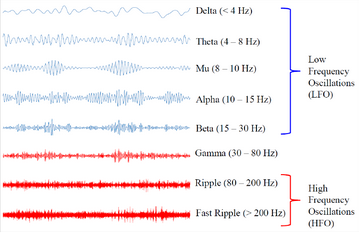
\includegraphics[width=0.6\textwidth]{assets/pics/frequency_band.png}
    \caption{Pita Frekuensi EEG pada rentang frekuensi tinggi dan rendah}
    \label{fig:2.2z}
\end{figure}
 

Sebelum dilakukan ekstraksi fitur dan klasifikasi, sinyal EEG umumnya melalui tahap \textit{preprocessing} untuk meningkatkan kualitas sinyal dan mengurangi gangguan yang tidak relevan. Tahapan ini biasanya meliputi \textit{filtering}, \textit{artifact removal}, \textit{baseline correction}, serta normalisasi atau standarisasi data \cite{eeg_feature_review}.


\textit{Filtering} adalah proses penyaringan sinyal untuk menghilangkan komponen frekuensi yang tidak berkaitan dengan aktivitas saraf serta mengurangi gangguan dari lingkungan seperti interferensi listrik serta gangguan yang muncul akibat pergerakan elektroda dan perubahan impedansi kulit. \textit{Filtering} dilakukan dengan membatasi rentang frekuensi sinyal menggunakan filter tertentu. Umumnya, \textit{band-pass filter} digunakan untuk mempertahankan frekuensi aktivitas otak, serta \textit{notch filter} untuk mereduksi interferensi jaringan listrik. Filter tambahan seperti \textit{high-pass filter} juga dapat digunakan untuk menghilangkan \textit{drift} sinyal berfrekuensi sangat rendah, sedangkan \textit{low-pass filter} digunakan untuk mereduksi komponen \textit{noise} berfrekuensi tinggi. Pemilihan filter perlu dilakukan secara hati-hati untuk menghindari distorsi sinyal atau pergeseran fase sinyal \cite{eeg_feature_review}. Pengaruh penggunaan filter terhadap sinyal EEG dapat dilihat pada ilustrasi \ref{fig:2.2}.


\begin{figure}[H]
    \centering
    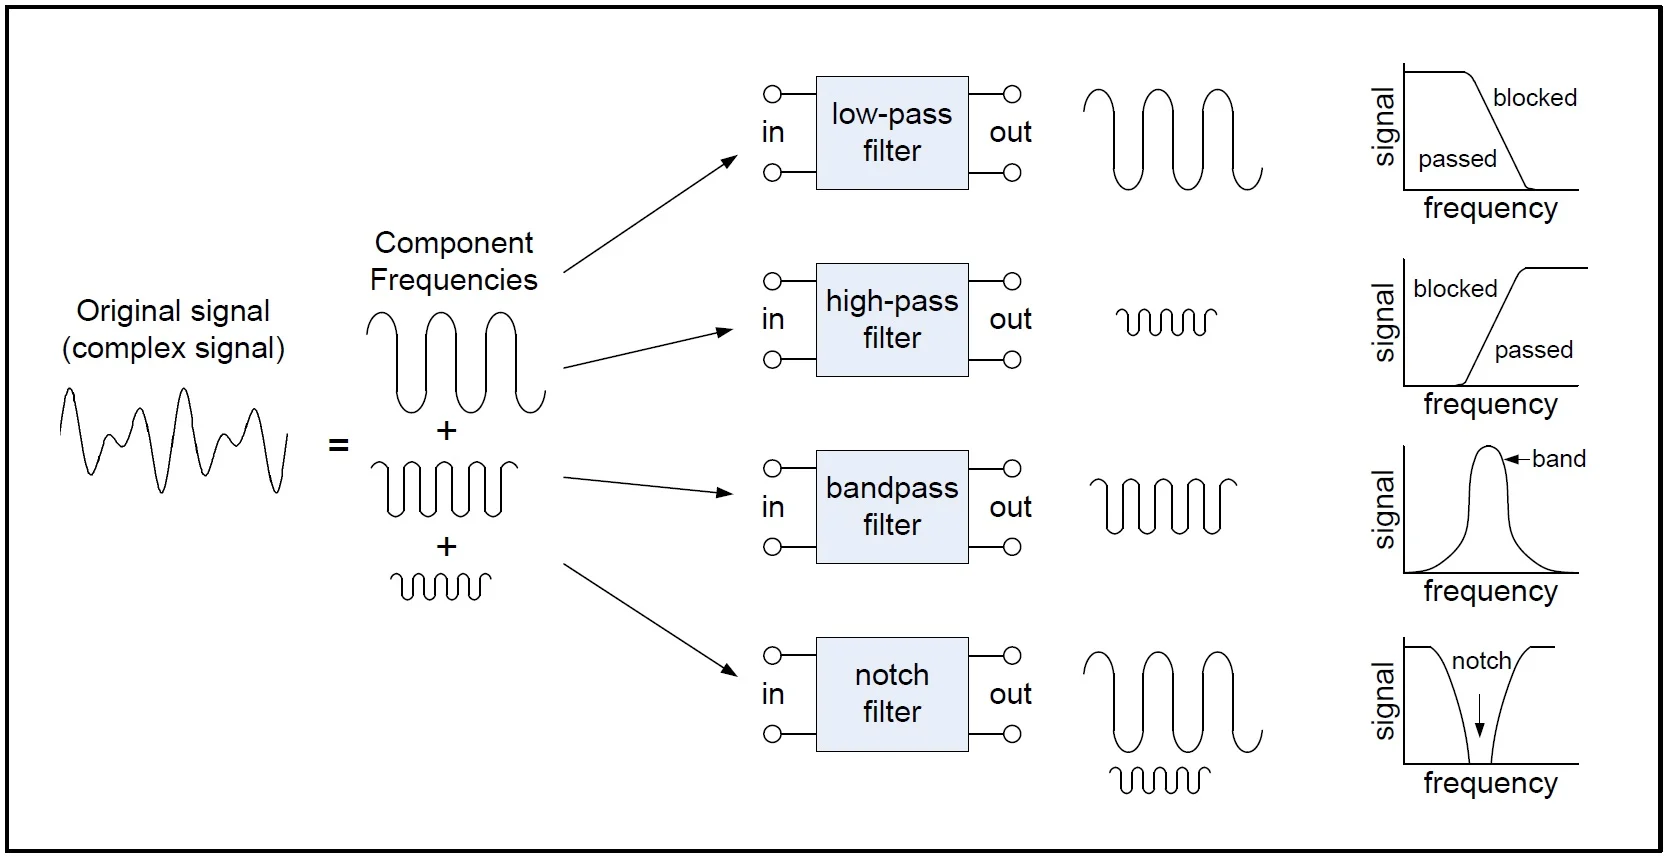
\includegraphics[width=\textwidth]{assets/pics/four_major_filters.png}
    \caption{Ilustrasi pengaruh berbagai jenis filter terhadap sinyal EEG}
    \label{fig:2.2}
\end{figure}

Sinyal EEG dapat terkontaminasi oleh artefak non-neural yang berasal dari aktivitas fisiologis maupun faktor eksternal. Artefak fisiologis umumnya disebabkan oleh kedipan mata dan pergerakan bola mata (\textit{electrooculogram}) dan aktivitas otot wajah dan kepala (\textit{electromyogram}), sedangkan artefak eksternal dapat berasal dari interferensi perangkat elektronik dan jaringan listrik. Keberadaan artefak dapat mempengaruhi kualitas sinyal, sebagaimana yang terlihat pada \ref{fig:2.3}, sehingga berpotensi menurunkan akurasi analisis maupun kinerja sistem klasifikasi. Berbagai metode digunakan untuk mengurangi artefak pada sinyal EEG, seperti \textit{Blind Source Separation} (BSS), \textit{Independent Component Analysis} (ICA), serta transformasi wavelet yang memungkinkan analisis pada domain waktu dan frekuensi untuk mendeteksi artefak \cite{eeg_feature_review}.

\begin{figure}[H]
    \centering
    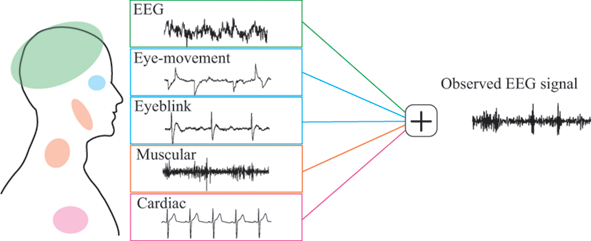
\includegraphics[width=0.6\textwidth]{assets/pics/artifact_eeg.png}
    \caption{Bentuk-Bentuk artefak pada sinyal EEG}
    \label{fig:2.3}
\end{figure}

Dalam analisis EEG berbasis \textit{machine learning}, normalisasi atau standarisasi digunakan untuk mengurangi variasi antar kanal maupun antar subjek yang menyebabkan perbedaan skala fitur dan mempengaruhi proses \textit{training}. Proses normalisasi digunakan untuk menyesuaikan skala fitur agar berada dalam rentang yang lebih seragam. Salah satu metode yang umum digunakan adalah \textit{Z-score normalization}, yaitu mengurangkan nilai rata-rata dan membaginya dengan standar deviasi sehingga data memiliki rata-rata nol dan variansi satu, sedangkan \textit{min-max normalization} juga dapat dilakukan dengan menskalakan nilai fitur ke dalam rentang tertentu, umumnya antara 0 dan 1. Proses ini memastikan kontribusi fitur lebih seimbang serta meningkatkan stabilitas dan kinerja model \cite{eeg_feature_review}.

\subsection{Feature Selection mRMR}
\label{Feature Selection mRMR}
Dalam aplikasi klasifikasi \textit{machine learning}, \textit{feature selection} merupakan langkah krusial untuk meminimalkan kesalahan klasifikasi. Secara formal, diberikan dataset $D$ yang terdiri dari $N$ sampel dan $M$ fitur $X = \{x_i \mid i = 1, 2, \dots, M\}$, serta variabel target $c$, maka seleksi fitur bertujuan menentukan subset berdimensi lebih rendah $R^m \subset R^M$ dengan $m < M$ yang mampu merepresentasikan target secara optimal\cite{mrmr_original}.

Secara umum, tujuan \textit{feature selection} dapat diformulasikan sebagai proses optimasi untuk mencari himpunan fitur $S \subseteq X$ dengan $|S| = m$ yang memaksimalkan ketergantungan terhadap kelas target. Ketergantungan ini seringkali diukur menggunakan \textit{mutual information} $I(S; c)$, sehingga permasalahan dapat dinyatakan sebagai:
\begin{equation}
\max_{S \subseteq X, |S| = m} I(S; c)
\end{equation}

Penggunaan seluruh fitur tidak selalu menghasilkan performa optimal karena adanya redundansi antar fitur. Fitur dengan korelasi tinggi cenderung memberikan informasi yang berulang, sehingga diperlukan metode \textit{feature selection} yang mempertimbangkan relevansi terhadap target sekaligus meminimalkan redundansi.

\textit{Minimum Redundancy Maximum Relevance} (mRMR) merupakan teknik seleksi fitur berbasis teori informasi yang memilih subset fitur dengan relevansi tinggi terhadap target dan redundansi rendah antar fitur.  Pendekatan ini efektif dalam mengurangi dimensi data tanpa mengorbankan informasi penting, sehingga meningkatkan efisiensi komputasi dan kemampuan generalisasi model \cite{sleep_apnea_eeg}\cite{tsmrmr_sleep}. Proses pemilihan fitur pada metode mRMR dilakukan secara iteratif dengan mengevaluasi keseimbangan antara relevansi fitur terhadap kelas target dan redundansi antar fitur yang telah dipilih sebelumnya. 

\begin{lstlisting}[
    style=modernpython,
    language=Python,
    caption={Algoritma mRMR untuk seleksi fitur.},
    label={code:mrmr-pseudocode}
]
# mRMR Feature Selection Algorithm

def mrmr_feature_selection(X, c, m):

    S = []                      # selected features
    F = X                       # candidate features

    # Select feature with maximum relevance
    for xi in F:
        relevance[xi] = MI(xi, c)

    x_best = argmax(relevance)

    S.append(x_best)
    F.remove(x_best)

    # Iterative feature selection
    while len(S) < m:

        for xj in F:

            rel = MI(xj, c)

            red = 0
            for xs in S:
                red += MI(xj, xs)

            red = red / len(S)

            score[xj] = rel - red

        x_best = argmax(score)

        S.append(x_best)
        F.remove(x_best)

    return S
\end{lstlisting}

Kode \ref{code:mrmr-pseudocode} menjelaskan proses seleksi fitur menggunakan metode \textit{Minimum Redundancy Maximum Relevance} (mRMR). Algoritma dimulai dengan memilih fitur yang memiliki nilai \textit{mutual information} tertinggi terhadap kelas target sebagai fitur awal. Selanjutnya, fitur lain dipilih secara iteratif berdasarkan nilai \textit{mRMR score}, yaitu selisih antara relevansi fitur terhadap target dan redundansinya terhadap fitur yang dipilih sebelumnya. Proses ini dilakukan hingga jumlah fitur terpilih mencapai jumlah yang diinginkan.

\subsection{Machine Learning untuk Klasifikasi ASD Berdasarkan Sinyal EEG}
\label{Klasifikasi Sinyal EEG dengan Machine Learning}

Dalam analisis EEG, \textit{machine learning} digunakan untuk mengklasifikasikan pola aktivitas otak berdasarkan fitur yang diekstraksi dari sinyal EEG. Fitur tersebut dapat berasal dari domain waktu, domain frekuensi, maupun domain waktu-frekuensi, dan digunakan untuk merepresentasikan karakteristik aktivitas neural yang berkaitan dengan kondisi fisiologis atau neurologis tertentu \cite{ml_eeg_fnirs_review}. Pendekatan ini telah digunakan pada berbagai aplikasi seperti deteksi kejang epilepsi, sistem \textit{brain-computer interface} (BCI), serta identifikasi pola aktivitas otak pada \textit{Autism Spectrum Disorder} (ASD) \cite{asd_eeg_abnormalities}.

Pada studi ASD, analisis EEG dalam domain frekuensi menjadi salah satu pendekatan yang umum digunakan karena aktivitas otak dapat direpresentasikan sebagai pola osilasi pada pita frekuensi tertentu \cite{eeg_asd_systematic}. Beberapa penelitian menunjukkan bahwa individu dengan ASD cenderung memiliki peningkatan daya pada pita delta, theta, beta, dan gamma, serta penurunan pada pita alpha. Pola ini dikenal sebagai \textit{U-shaped spectral profile} dan digunakan untuk merepresentasikan abnormalitas aktivitas neural pada ASD sebagaimana diilustrasikan pada ilustrasi \ref{fig:ushape}. \cite{asd_eeg_abnormalities}.

\begin{figure}[H]
    \centering
    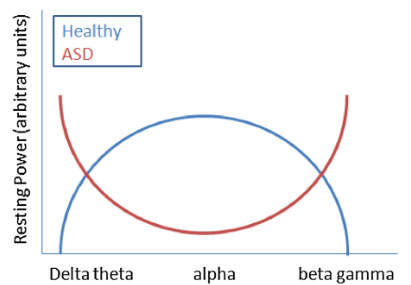
\includegraphics[width=0.5\textwidth]{assets/pics/ushaped.png}
    \caption{Ilustrasi \textit{U-shaped spectral profile} yang ditemukan pada pita frekuensi penderita ASD}
    \label{fig:ushape}
\end{figure}

Berdasarkan fitur yang diperoleh, proses klasifikasi dilakukan menggunakan algoritma \textit{machine learning} untuk membangun model prediksi. Berbagai metode seperti \textit{support vector machine} (SVM), \textit{k-nearest neighbor} (KNN), dan \textit{random forest} telah banyak digunakan dalam klasifikasi EEG dan menunjukkan performa yang baik dalam mengenali pola aktivitas neural yang kompleks \cite{ml_eeg_fnirs_review}. Meskipun pendekatan \textit{deep learning} berkembang pesat, metode \textit{machine learning} konvensional masih relevan terutama pada kondisi data terbatas dan kebutuhan interpretabilitas model \cite{ml_eeg_classification}.

\begin{figure}[H]
    \centering
    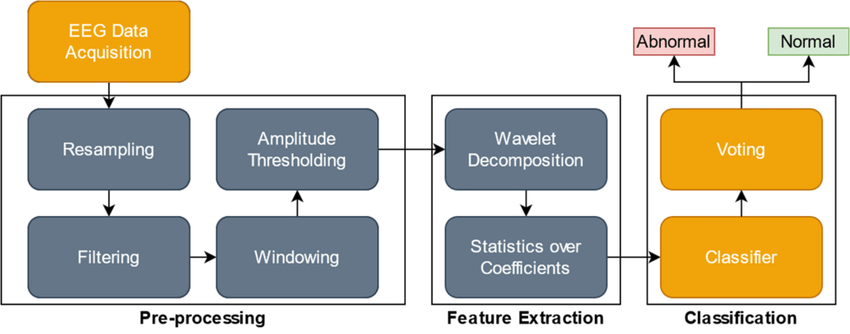
\includegraphics[width=0.8\textwidth]{assets/pics/general_pipeline.png}
  \caption{Ilustrasi umum pipeline klasifikasi ASD berbasis sinyal EEG}
    \label{fig:pipeline_asd_classification}
\end{figure}

Gambar \ref{fig:pipeline_asd_classification} menunjukkan proses klasifikasi berbasis sinyal EEG pada umumnya. Pipeline diawali akuisisi sinyal EEG, dilanjutkan dengan tahap \textit{preprocessing} untuk meningkatkan kualitas sinyal sebelum dianalisis lebih lanjut. Setelah itu, dilakukan proses ekstraksi fitur untuk memperoleh representasi informasi dari sinyal EEG yang relevan terhadap proses klasifikasi. Fitur yang diperoleh dari tahap ekstraksi kemudian digunakan sebagai masukan bagi model \textit{machine learning} untuk mempelajari pola-pola dalam sinyal EEG dan melakukan proses klasifikasi berupa prediksi terhadap kelas atau label yang telah ditentukan sesuai dengan tujuan penelitian. Secara umum, pipeline ini bertujuan mengubah sinyal EEG mentah menjadi representasi fitur yang lebih informatif dan terstruktur sehingga dapat diproses secara efektif oleh algoritma klasifikasi.

\subsection{Augmentasi Data EEG}
\label{Augmentasi Data EEG}
Performa model \textit{machine learning} sangat dipengaruhi oleh jumlah, kualitas, dan keragaman data \textit{training}. Pada analisis sinyal EEG, keterbatasan data menjadi tantangan karena proses akuisisi relatif mahal, memakan waktu, serta menghasilkan data dengan variabilitas tinggi antar individu maupun sesi \cite{cross_dataset_eeg}. Variabilitas tersebut dipengaruhi oleh perbedaan perangkat, konfigurasi kanal, kondisi eksperimen, aktivitas fisiologis, dan artefak non-neural, sehingga distribusi data EEG menjadi kompleks dan tidak konsisten antar dataset. Kondisi ini dapat menyebabkan model mengalami \textit{overfitting} dan memiliki kemampuan generalisasi yang rendah terhadap data baru.

Untuk mengatasi permasalahan tersebut, berbagai penelitian mengusulkan penggunaan teknik \textit{data augmentation} untuk meningkatkan jumlah dan variasi data \textit{training} tanpa memerlukan proses perekaman tambahan \cite{eeg_augmentation_review}. Secara umum, \textit{data augmentation} bertujuan menghasilkan sampel data baru yang tetap mempertahankan karakteristik utama data asli sehingga model dapat mempelajari representasi pola yang lebih stabil.

Pada sinyal \textit{time-series} seperti sinyal EEG, augmentasi konvensional umumnya dilakukan melalui manipulasi langsung terhadap sinyal dalam domain waktu maupun frekuensi \cite{traditional_timeseries_aug}. Pendekatan ini menghasilkan sampel baru dengan memodifikasi data asli menggunakan aturan transformasi tertentu tanpa mempelajari distribusi data secara eksplisit. Beberapa metode augmentasi yang umum digunakan pada data \textit{time-series} meliputi \textit{Flipping}, \textit{Down-sampling}, \textit{Adding Slope}, \textit{Amplitude Adjusted Fourier Transform (AAFT)}, \textit{Iterative Amplitude Adjusted Fourier Transform (IAAFT)}, \textit{Amplitude-Phase Perturbation (APP)}, dan \textit{Short-Time Fourier Transform (STFT)-based Augmentation}. Ilustrasi penerapan masing-masing metode ditunjukkan pada gambar \ref{fig:traditional_augmentation_example} dengan detail implementasi yang disajikan pada tabel \ref{tab:traditional_augmentation_methods}.

\begin{figure}[H]
    \centering
    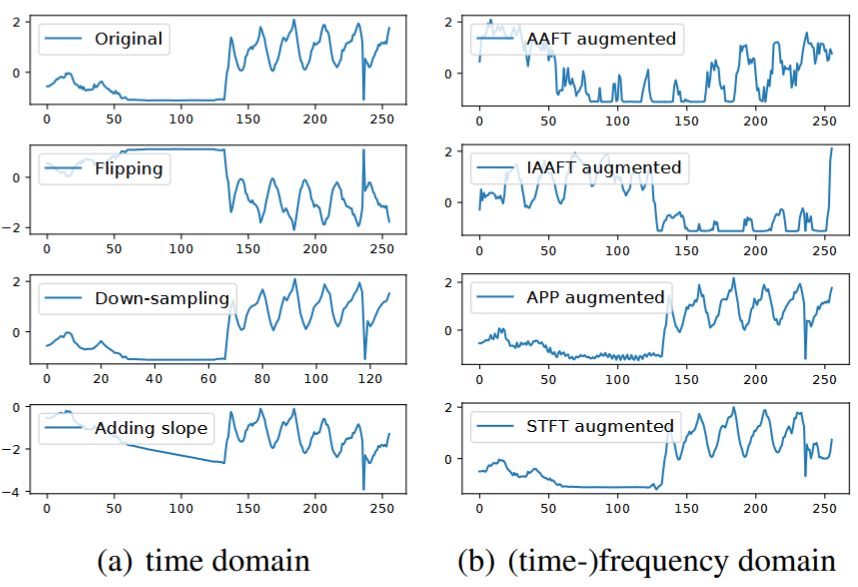
\includegraphics[width=\textwidth]{assets/pics/traditional_augmentation.png}
    \caption{Ilustrasi metode augmentasi pada data \textit{time-series}}
    \label{fig:traditional_augmentation_example}
\end{figure}

\begin{table}[H]
\centering
\footnotesize
\caption{Metode augmentasi pada data \textit{time-series}}
\label{tab:traditional_augmentation_methods}
\begin{tabular}{|c|c|p{6cm}|}
\hline
\textbf{Metode} & \textbf{Formula} & \textbf{Pengaruh terhadap Data} \\ \hline

\textit{Flipping} &
$x'(t) = -x(t)$ &
Membalik amplitudo sinyal terhadap sumbu horizontal sehingga pola temporal tetap terjaga tetapi orientasi sinyal berubah. \\ \hline

\textit{Down-sampling} &
$x'(t) = x(nt)$ &
Mengurangi jumlah sampel dengan faktor tertentu sehingga menghasilkan variasi resolusi temporal data. \\ \hline

\textit{Adding Slope} &
$x'(t) = x(t) + \alpha t$ &
Menambahkan tren linier pada sinyal untuk mensimulasikan perubahan gradual atau \textit{drift}. \\ \hline

\textit{AAFT} &
$x'(t)=\mathcal{F}^{-1}\!\left(|X(f)|e^{j\phi_r(f)}\right)$ &
Menghasilkan sinyal surrogate yang mempertahankan distribusi amplitudo dan spektrum daya secara aproksimatif. \\ \hline

\textit{IAAFT} &
$x'(t)=\mathrm{IAAFT}(x(t))$ &
Menghasilkan sinyal surrogate yang lebih akurat dalam mempertahankan distribusi amplitudo dan spektrum daya dibandingkan AAFT melalui proses iteratif. \\ \hline

\textit{APP} &
$X'(f)=A(f)e^{j(\phi(f)+\Delta\phi)}$ &
Menambahkan perturbasi pada amplitudo atau fase di domain frekuensi untuk menciptakan variasi sinyal yang realistis. \\ \hline

\textit{STFT-based Augmentation} &
$X'(m,\omega)=\mathrm{Aug}(X(m,\omega))$ &
Melakukan augmentasi pada representasi waktu-frekuensi sehingga karakteristik lokal sinyal dapat dimodifikasi tanpa mengubah struktur global secara signifikan. \\ \hline

\end{tabular}
\end{table}


Meskipun relatif sederhana dan mudah diterapkan, metode augmentasi konvensional memiliki keterbatasan dalam mempertahankan karakteristik kompleks sinyal EEG secara menyeluruh. Transformasi langsung terhadap sinyal berpotensi mengubah dependensi spasial maupun temporal yang penting dalam representasi aktivitas fisiologis. Selain itu, beberapa penelitian menunjukkan bahwa augmentasi sederhana tidak selalu meningkatkan performa model klasifikasi EEG secara konsisten. Oleh karena itu, penelitian lain mulai menggunakan pendekatan berbasis model generatif yang mampu mempelajari distribusi data untuk menghasilkan sampel sintetis yang lebih representatif terhadap karakteristik sinyal EEG.

\subsection{Model Generatif untuk Augmentasi Data}
\label{sec:model_generatif}

Model generatif merupakan pendekatan dalam \textit{machine learning} yang mempelajari distribusi dan pola suatu dataset untuk menghasilkan sampel data baru yang memiliki karakteristik serupa dengan data asli, berbeda dengan model diskriminatif yang digunakan pada proses klasifikasi atau prediksi label \cite{generative_models_survey}. Model generatif digunakan dalam berbagai aplikasi seperti sintesis gambar, rekonstruksi data (\textit{data reconstruction}), pemrosesan suara, hingga pembuatan data sintetis untuk kebutuhan \textit{training} model.

Data sintetis yang dihasilkan model generatif menjadi salah satu solusi terhadap berbagai permasalahan pada proses pengolahan data, seperti keterbatasan jumlah data, ketidakseimbangan kelas (\textit{class imbalance}), serta kendala privasi dan akuisisi data \cite{generative_models_survey}. Dalam konteks \textit{machine learning}, data sintetis yang dihasilkan oleh model generatif dapat digunakan sebagai bentuk \textit{data augmentation} untuk meningkatkan jumlah dan keragaman data \textit{training} tanpa memerlukan proses pengumpulan data baru secara langsung. Pendekatan ini memungkinkan model mempelajari representasi data yang lebih beragam sehingga dapat membantu meningkatkan kemampuan generalisasi model.

Berbagai arsitektur model generatif telah dikembangkan dalam penelitian \textit{deep learning}. Beberapa pendekatan yang umum digunakan meliputi \textit{Generative Adversarial Networks} (GAN), \textit{Variational Autoencoders} (VAE), serta model berbasis difusi (\textit{diffusion models}). Masing-masing pendekatan memiliki mekanisme pembelajaran dan karakteristik yang berbeda dalam menghasilkan data sintetis.

    \begin{table}[H]
    \centering
    \footnotesize
\caption{Perbandingan karakteristik, kelebihan, dan keterbatasan beberapa model generatif utama}
    \label{tab:generative_models}
    \begin{tabular}{|c|p{4cm}|p{5cm}|}
    \hline
    \textbf{Model} & \textbf{Karakteristik Utama} & \textbf{Kelebihan dan Keterbatasan} \\ \hline

    GAN &
    Menggunakan mekanisme kompetitif antara generator dan discriminator untuk menghasilkan data sintetis. &
    Mampu menghasilkan data yang realistis, namun proses \textit{training} cenderung tidak stabil dan rentan terhadap \textit{mode collapse}. \\ \hline

    VAE &
    Mempelajari distribusi laten probabilistik melalui arsitektur encoder-decoder. &
    Memiliki proses \textit{training} yang lebih stabil dan mampu menghasilkan representasi laten yang terstruktur, namun kualitas data sintetis dapat lebih halus dibanding GAN. \\ \hline

    Diffusion Model &
    Menghasilkan data melalui proses denoising bertahap dari distribusi acak. &
    Mampu menghasilkan kualitas data yang tinggi, namun memerlukan kompleksitas komputasi dan waktu \textit{training} yang lebih besar. \\ \hline

    \end{tabular}
    \end{table}

Dalam analisis sinyal EEG, model generatif digunakan untuk menghasilkan data sintetis yang mengikuti distribusi statistik data asli. Pendekatan ini memungkinkan model mempelajari struktur laten dari sinyal EEG sehingga data sintetis yang dihasilkan dapat mempertahankan karakteristik temporal maupun spasial yang penting dalam proses klasifikasi. Beberapa penelitian menunjukkan bahwa penggunaan data sintetis dari model generatif dapat membantu meningkatkan performa dan kemampuan generalisasi model klasifikasi EEG, terutama pada kondisi jumlah data \textit{training} yang terbatas \cite{gan_eeg_emotion}.

Salah satu model generatif yang banyak digunakan dalam augmentasi data EEG adalah \textit{Variational Autoencoder} (VAE). Dibandingkan GAN, VAE memiliki proses \textit{training} yang lebih stabil dan tidak bergantung pada mekanisme adversarial yang rentan terhadap \textit{mode collapse}. Selain itu, dibandingkan \textit{diffusion model}, VAE umumnya memerlukan kompleksitas komputasi dan jumlah data \textit{training} yang lebih rendah. Karakteristik tersebut menjadikan VAE lebih sesuai untuk penelitian ini yang menggunakan dataset EEG dengan jumlah data terbatas\cite{eeg_augmentation_review}.   


\subsection{Variational Auto Encoder}
\label{Variational AutoEncoder}
\textit{Variational Autoencoder} (VAE) merupakan salah satu model generatif berbasis \textit{deep learning} yang digunakan untuk mempelajari representasi laten dari suatu dataset dan menghasilkan sampel data baru dengan karakteristik yang serupa dengan data asli. Berbeda dengan \textit{autoencoder} konvensional yang berfokus pada proses kompresi dan rekonstruksi data, VAE memodelkan representasi laten sebagai distribusi probabilistik sehingga memungkinkan proses generasi data baru melalui ruang laten (\textit{latent space}) yang dipelajari oleh model \cite{cvae_gan_eeg}.

\begin{figure}[H]
    \centering
    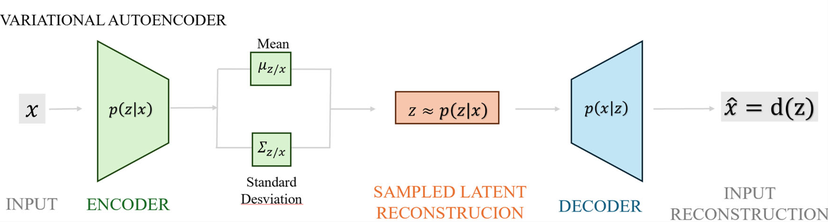
\includegraphics[width=0.8\textwidth]{assets/pics/vae-architecture.png}
    \caption{Arsitektur umum \textit{Variational Autoencoder} (VAE)}
    \label{fig:vae_architecture}
\end{figure}


Arsitektur VAE terdiri atas dua komponen utama, yaitu \textit{encoder} dan \textit{decoder}, seperti yang diilustrasikan pada Gambar \ref{fig:vae_architecture}. \textit{Encoder} bertugas memetakan data input ke representasi laten berdimensi lebih rendah dalam bentuk parameter distribusi probabilistik, yaitu nilai rata-rata ($\mu$) dan variansi ($\sigma$). Representasi laten tersebut kemudian digunakan oleh \textit{decoder} untuk merekonstruksi kembali data sehingga menghasilkan output yang memiliki karakteristik serupa dengan data asli.

Proses \textit{training} VAE dilakukan menggunakan fungsi objektif \textit{Evidence Lower Bound} (ELBO), yang terdiri atas dua komponen utama, yaitu \textit{reconstruction loss} dan \textit{Kullback--Leibler Divergence} (KL Divergence). \textit{Reconstruction loss} digunakan untuk mengukur kualitas hasil rekonstruksi data, sedangkan KL Divergence berfungsi menjaga distribusi laten agar tetap mendekati distribusi normal standar. Secara matematis, fungsi objektif VAE dirumuskan sebagaimana pada persamaan \ref{eq:elbo}:
\begin{equation}
\mathcal{L}(\theta, \phi; x) =
\mathbb{E}_{q_{\phi}(z|x)}[\log p_{\theta}(x|z)] -
D_{KL}(q_{\phi}(z|x) \parallel p(z))
\label{eq:elbo}
\end{equation}
di mana $q_{\phi}(z|x)$ merepresentasikan distribusi laten yang dihasilkan oleh \textit{encoder}, $p_{\theta}(x|z)$ merepresentasikan proses rekonstruksi oleh \textit{decoder}, dan $p(z)$ merupakan distribusi prior pada ruang laten. Komponen pertama pada persamaan tersebut merepresentasikan kualitas rekonstruksi data, sedangkan komponen kedua berfungsi sebagai regularisasi untuk menjaga struktur distribusi laten \cite{vae_original}.

Proses \textit{sampling} pada ruang laten tidak dapat dilakukan secara langsung dalam proses \textit{training} menggunakan metode \textit{backpropagation}. Oleh karena itu, VAE menggunakan teknik yang dikenal sebagai \textit{reparameterization trick}. Melalui teknik ini, variabel laten $z$ dinyatakan sebagaimana yang terlihat pada persamaan \ref{eqz}. 
\begin{equation}
z = \mu + \sigma \cdot \epsilon
\label{eqz}
\end{equation}

di mana $\epsilon$ merupakan variabel acak yang diambil dari distribusi normal standar $\mathcal{N}(0,1)$. Dengan pendekatan ini, proses \textit{sampling} dapat ditransformasikan menjadi operasi deterministik yang memungkinkan gradien tetap dapat dihitung selama proses \textit{training} neural network \cite{vae_original}.


\subsection{Metode Evaluasi Data Sintetis Sinyal EEG}

Evaluasi kualitas data sintetis diperlukan untuk menilai sejauh mana sinyal EEG yang dihasilkan model generatif mampu mempertahankan karakteristik data asli. Dalam penelitian referensi \cite{eeg_gan}, evaluasi dilakukan menggunakan beberapa metrik kuantitatif yang umum digunakan pada model generatif, yaitu, \textit{Frechet Inception Distance} (FID), \textit{Euclidean Distance} (ED), dan \textit{Sliced Wasserstein Distance} (SWD). Definisi, formulasi matematis, serta aspek kualitas data yang dievaluasi oleh masing-masing metrik dirangkum dalam tabel \ref{tab:evaluation_metrics}.

\begin{table}[H]
\centering
\footnotesize
\caption{Metrik evaluasi data sintetis EEG}
\label{tab:evaluation_metrics}
\renewcommand{\arraystretch}{1.5}
\resizebox{\textwidth}{!}{
\begin{tabular}{|c|p{6cm}|p{5cm}|}
\hline
\textbf{Metrik} & \textbf{Formula} & \textbf{Aspek yang Dievaluasi} \\ \hline

\textit{Frechet Inception Distance} (FID) &
$\displaystyle
\|\mu_r-\mu_g\|^2 +
Tr(\Sigma_r+\Sigma_g
-2(\Sigma_r\Sigma_g)^{1/2})
$
&
Mengukur kesamaan distribusi fitur antara data asli dan sintetis. \\ \hline

\textit{Euclidean Distance} (ED) &
$\displaystyle
d(x,y)=
\sqrt{
\sum_{i=1}^{n}(x_i-y_i)^2
}
$
&
Mengukur kemiripan langsung antar sampel data asli dan sintetis. \\ \hline

\textit{Sliced Wasserstein Distance} (SWD) &
$\displaystyle
SWD(P,Q)=
\int_{\theta}
W_1(P_{\theta},Q_{\theta})
\, d\theta
$
&
Mengukur kesamaan distribusi global melalui proyeksi satu dimensi. \\ \hline

\end{tabular}
}
\end{table}

Penelitian referensi \cite{eeg_gan} menunjukkan bahwa tidak terdapat satu metrik yang mampu merepresentasikan seluruh karakteristik kualitas sinyal EEG sintetis secara menyeluruh. Pada penelitian tersebut, nilai FID yang rendah tidak selalu menunjukkan kesamaan karakteristik spasial dan spektral terhadap data asli, sedangkan SWD dinilai lebih mampu merepresentasikan distribusi sinyal yang natural. Oleh karena itu, penggunaan beberapa metrik evaluasi secara bersamaan diperlukan untuk memperoleh penilaian kualitas data sintetis yang lebih komprehensif.

\section{Penelitian Terdahulu}
\label{Penelitian Terdahulu}

Berbagai penelitian telah mengusulkan pendekatan \textit{machine learning} untuk klasifikasi \textit{Autism Spectrum Disorder} (ASD) berbasis sinyal EEG dengan memanfaatkan karakteristik aktivitas neural sebagai fitur klasifikasi. Selain itu, beberapa penelitian juga menerapkan teknik augmentasi data untuk mengatasi keterbatasan jumlah data \textit{training} dan meningkatkan performa model klasifikasi.

Tinjauan terhadap penelitian terdahulu diperlukan untuk memahami perkembangan metode klasifikasi EEG, pendekatan augmentasi data yang telah digunakan, serta keterbatasan yang masih menjadi tantangan dalam pengembangan sistem klasifikasi ASD berbasis EEG.

\subsection{Klasifikasi ASD Berbasis EEG Menggunakan Kombinasi mRMR dan XGBoost}
\label{Klasifikasi ASD Berbasis EEG Menggunakan mRMR dan XGBoost}

Pada penelitian rujukan \cite{paper_ref}, klasifikasi \textit{Autism Spectrum Disorder} (ASD) dilakukan menggunakan sinyal EEG dengan memanfaatkan seleksi fitur dan algoritma \textit{machine learning}. Penelitian berfokus pada penggunaan fitur domain frekuensi untuk merepresentasikan karakteristik aktivitas neural yang berkaitan dengan ASD serta meningkatkan performa klasifikasi melalui pemilihan fitur yang optimal.

Penelitian menggunakan metode \textit{minimum Redundancy Maximum Relevance} (mRMR) untuk memilih fitur yang paling relevan dan memiliki redundansi minimum antar fitur. Sebelum proses seleksi fitur, sinyal EEG melalui tahap \textit{preprocessing} seperti segmentasi, \textit{filtering}, dan dekomposisi pita frekuensi. Fitur hasil seleksi kemudian digunakan sebagai masukan bagi model klasifikasi berbasis \textit{ensemble}, yaitu XGBoost. Performa metode tersebut dibandingkan dengan model \textit{Deep Neural Network} (DNN) sebagai metode \textit{baseline}, sehingga peningkatan performa yang diperoleh dievaluasi berdasarkan hasil perbandingan terhadap model DNN.

Hasil penelitian menunjukkan bahwa kombinasi mRMR dan XGBoost mampu memberikan performa klasifikasi yang baik dalam membedakan individu ASD dan non-ASD. Penggunaan mRMR membantu meningkatkan kualitas fitur, sementara XGBoost memberikan kemampuan klasifikasi yang robust terhadap kompleksitas data EEG. Namun, penelitian juga menunjukkan bahwa pendekatan tersebut memiliki waktu komputasi yang lebih tinggi dibandingkan model dasar yang digunakan sebagai pembanding. Selain itu, penelitian masih dilakukan pada jumlah dataset yang relatif terbatas, sehingga kemampuan generalisasi model masih menjadi tantangan dalam pengembangan sistem klasifikasi EEG berbasis ASD. 

\subsection{Metode Augmentasi Data pada Sinyal EEG Menggunakan Variational Autoencoder}
\label{Augmentasi Data pada Sinyal EEG Menggunakan Variational Autoencoder}

Pada penelitian rujukan \cite{gan_eeg_emotion}, digunakan pendekatan augmentasi data berbasis \textit{Variational Autoencoder} (VAE) untuk menghasilkan sinyal EEG sintetis pada tugas klasifikasi \textit{motor imagery}. Penelitian memanfaatkan BCI Competition IV Dataset 2a yang terdiri dari data EEG 22 kanal dari 9 subjek. Data EEG direpresentasikan dalam bentuk matriks dua dimensi untuk menyesuaikan penggunaan arsitektur berbasis \textit{2D Convolutional Neural Network} (2D CNN).

Model VAE terdiri dari komponen \textit{encoder} dan \textit{decoder} yang digunakan untuk mempelajari representasi laten dari sinyal EEG dan merekonstruksi kembali data sintetis yang menyerupai data asli. Untuk evaluasi klasifikasi, penelitian menggunakan arsitektur EEGNet dan membandingkan performa model yang dilatih menggunakan data asli dengan model yang dilatih menggunakan data hasil augmentasi.

Hasil penelitian menunjukkan bahwa penggunaan data sintetis dari VAE mampu meningkatkan performa klasifikasi secara signifikan, di mana akurasi meningkat dari 0.73 menjadi 0.88. Peningkatan juga terlihat pada metrik \textit{precision}, \textit{recall}, dan \textit{f1-score}, yang menunjukkan bahwa data sintetis mampu memperkaya variasi data \textit{training}.

Namun, penelitian tersebut masih berfokus pada representasi sinyal EEG dalam domain waktu dan belum mempertimbangkan karakteristik domain frekuensi secara menyeluruh. Padahal, analisis domain frekuensi memiliki peran penting dalam identifikasi pola neurofisiologis pada EEG, termasuk pada studi ASD, karena informasi aktivitas neural banyak direpresentasikan melalui distribusi daya pada pita frekuensi tertentu.

\subsection{Dataset EEG yang Digunakan dalam Penelitian}
\label{Dataset EEG yang Digunakan}

Dataset yang digunakan dalam penelitian ini berupa sinyal \textit{electroencephalogram} (EEG) dari studi rujukan \cite{eeg_dataset_asd}, yang terdiri dari data subjek dengan dan tanpa diagnosis \textit{Autism Spectrum Disorder} (ASD). Dataset ini digunakan karena mampu merepresentasikan karakteristik aktivitas neural yang berkaitan dengan ASD sehingga relevan untuk pengembangan model klasifikasi berbasis \textit{machine learning}.

Data EEG dikumpulkan dari sepuluh partisipan yang terdiri dari lima anak dengan ASD berusia 6--10 tahun dan lima subjek kontrol sehat. Akuisisi dilakukan menggunakan perangkat \textit{OpenBCI Cyton Biosensing Board} dengan 16 kanal EEG berdasarkan sistem \textit{International 10--20 System}. Proses perekaman dilakukan tanpa stimulus eksternal dengan upaya meminimalkan distraksi partisipan untuk menjaga kualitas sinyal EEG yang diperoleh.

Setelah akuisisi, sinyal EEG melalui tahap \textit{preprocessing} menggunakan metode seperti \textit{Butterworth filtering}, \textit{Discrete Wavelet Transform} (DWT), dan \textit{Independent Component Analysis} (ICA) untuk mengurangi artefak dan meningkatkan kualitas sinyal \cite{paper_ref}. Selanjutnya, sinyal diproses melalui segmentasi dan dekomposisi ke dalam pita frekuensi utama seperti delta, theta, alpha, beta, dan gamma untuk proses ekstraksi fitur dan klasifikasi.

Meskipun dataset ini relevan untuk analisis ASD berbasis EEG, jumlah partisipan yang relatif kecil menjadi salah satu keterbatasan penelitian. Dataset hanya mencakup data dari sepuluh subjek sehingga berpotensi membatasi kemampuan generalisasi model serta meningkatkan risiko \textit{overfitting}, khususnya pada model \textit{machine learning} yang memerlukan jumlah data \textit{training} yang lebih besar.

\section{Fokus pada Celah Penelitian}
\label{Fokus pada Celah Penelitian}

Berdasarkan tinjauan pustaka yang telah dilakukan, terdapat celah penelitian dalam pemanfaatan teknik augmentasi data berbasis \textit{Variational Autoencoder} (VAE) untuk analisis sinyal EEG. Beberapa penelitian sebelumnya telah menerapkan VAE untuk menghasilkan data EEG sintetis, khususnya dalam konteks tugas klasifikasi berbasis \textit{motor imagery} menggunakan arsitektur seperti \textit{2D Convolutional Neural Network} (CNN). Pendekatan tersebut menunjukkan bahwa data sintetis mampu meningkatkan performa model klasifikasi dengan memperkaya variasi data \textit{training}. Meskipun demikian, fokus penelitian masih terbatas pada representasi sinyal dalam domain waktu atau spasial, tanpa mengeksplorasi secara mendalam karakteristik sinyal dalam domain frekuensi.

Di sisi lain, analisis berbasis domain frekuensi memiliki peran penting dalam studi EEG, terutama dalam mengidentifikasi pola osilasi neural yang berkaitan dengan kondisi neurologis seperti \textit{Autism Spectrum Disorder} (ASD). Pemanfaatan data sintetis berbasis VAE pada representasi fitur frekuensi masih relatif terbatas, dan belum banyak dilakukan pengkajian terkait pengaruh augmentasi sinyal EEG terhadap kualitas fitur dan performa model klasifikasi berbasis \textit{machine learning} konvensional.

Oleh karena itu, penelitian ini mengusulkan pendekatan yang mengintegrasikan teknik augmentasi data berbasis VAE dengan ekstraksi fitur domain frekuensi, serta memanfaatkan metode seleksi fitur \textit{minimum Redundancy Maximum Relevance} (mRMR) dan algoritma klasifikasi \textit{XGBoost}. Pendekatan ini bertujuan untuk mengeksplorasi bagaimana data sintetis yang dihasilkan pada domain frekuensi dapat meningkatkan kualitas representasi fitur serta performa klasifikasi ASD. Dengan mengisi celah ini, diharapkan penelitian ini dapat memberikan kontribusi dalam pengembangan metode klasifikasi EEG yang lebih robust dan akurat, khususnya pada kondisi dataset yang terbatas.

